In order to distribute the work among several threads I decided to split the input file into blocks, one per thread, so that the work will be split and distributed equally. This allows to reach the maximum speedup because all the threads will have some work to do and none of them will finish a lot earlier than any other and stop without doing nothing.

\begin{figure}[H]
\centering
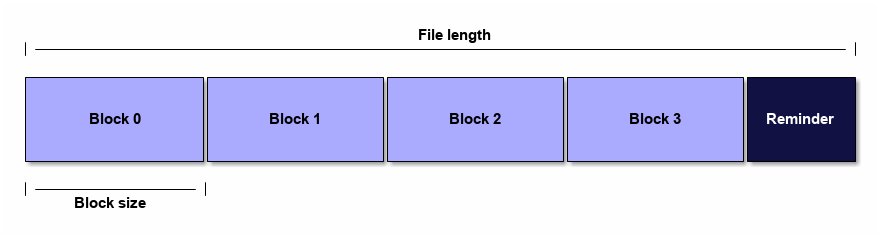
\includegraphics[scale = 0.4]{./Pictures/multithreading} % x compreso tra 0 e 1
\caption{Block subdivision}
\label{fig:multithreading}
\end{figure}

The block size is adjusted in order to be a multiple of 64 bits (the size of the Blowfish's block size), in this way we have a small reminder at the end which we have to handle, I choose to do so in the main thread with a specific portion of code different from the thread's one which may remain neat. Without this adjustment we would had to deal with the reminder of every thread, this would make the code less clean and uselessly complex.\\
In the end the behavior is the following: after the preliminary setup the threads are created, every thread autonomously read the respective portion of the input file 64 bits at a time, encrypt it and write the result in the output file. In the meanwhile the main thread work on the reminder in a similar way, except for a detail, the last 64 bits block.

\section{Padding}
The problem is this: the Blowfish algorithm works only on a fixed size block of 64 bits, but it's unlikely that the input file size is exactly divisible by 8 bytes (64 bits), so once we reach the last block we have to be sure to fill it in some way to make it the right size, the so called \emph{padding} operation.\\
There are several well known ways to handle the padding like to fill with zeros, but most of them make it difficult to distinguish the padding from the actual user data while decrypting. The best protocol I found to deal with this problem is to fill the remaining bytes with the number of bytes to fill, this means embedding the information about the padding size in the padding itself, so we will always be able to correctly decode and trim the output file, an example in figure \ref{fig:padding}.

\begin{figure}[H]
\centering
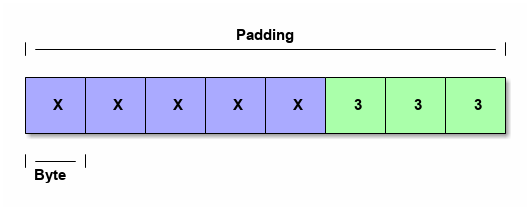
\includegraphics[scale = 0.5]{./Pictures/padding} % x compreso tra 0 e 1
\caption{Padding example (three bytes to be filled)}
\label{fig:padding}
\end{figure}

\subparagraph{Corner case}
One last thing to be noted is the case in which there is no need of padding, since while decoding we read the last byte to know the padding length, the padding cannot be of length zero, because otherwise, we would have no means to know if actually there is a padding or not. So the rule is that there must always be at least one byte of padding.\\
Now we have to find a way to handle the case in which there is no need to pad (length zero), the only way (that come naturally from the implementation) is to add an entire byte of padding, which will be composed of 8s as in figure \ref{fig:padding8}.

\begin{figure}[H]
\centering
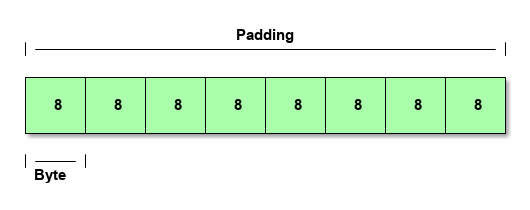
\includegraphics[scale = 0.5]{./Pictures/padding8} % x compreso tra 0 e 1
\caption{Corner case}
\label{fig:padding8}
\end{figure}